%*****************************************
\chapter{Advanced Topics}\label{ch08:topics}
%*****************************************

% This will cover the various statistics functions, the stat-pack addin, and dealing with ``dirty'' input data.

Excel includes many advanced features not covered elsewhere in this book and they were gathered in this final chapter. Most of these features are only occasionally used but when needed, they provide an essential resource.

\section{Database Functions}

\begin{center}
	\begin{objbox}{Learning Objectives}
		\begin{itemize}
			\setlength{\itemsep}{0pt}
			\setlength{\parskip}{0pt}
			\setlength{\parsep}{0pt}
			
			\item Excel provides several functions that make a spreadsheet behave more like a database.
		\end{itemize}
	\end{objbox}
\end{center}

A database is a collection of data that is used by business leadership to support decisions. A database is commonly used to contain personnel, supply, manufacturing, sales and many other types of information. A database is normally created with a program like Microsoft Access, but that program is complex with a steep learning curve. Simple data tables with a few database properties can be created and manipulated in Excel, as shown in this section.

\subsection{Create a Data Table}

\begin{enumerate}
	\item Open workbook \fmtWorkbookName{CH9-Database.xlsx}
	\item This workbook has only one worksheet, \fmtWorksheetName{Sales}.
	\item Save the workbook as \fmtWorkbookName{CH9-Sales.xlsx}.
\end{enumerate}

This worksheet contains the May, $ 2020 $, sales report for \textit{MongoSales Corp}. The report includes the sales representative name, the district, name, and zip for the company that purchased items, the date of the purchase, the item purchased, the number of units purchased, price per unit, and total sale value. (\textit{Note}: this is dummy data.) The worksheet needs to be converted to a table in order to use it as a database.

\begin{enumerate}[resume]
	\item Click cell \fmtCellLocation{A1} to activate that cell.
	\item Click \fmtRibbonButton{Insert $ \Rightarrow $ Tables $ \Rightarrow $ Table}.
	\item Excel automatically selects cells \fmtCellLocation{\$A\$1:\$I\$69}, which is the entire dataset. Be certain \fmtPopupButton{My table has headers} is checked (Figure \ref{09:fig10}).

	\begin{figure}[H]
		\centering
		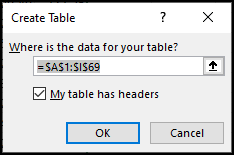
\includegraphics[width=\maxwidth{.95\linewidth}]{gfx/ch09_fig10}
		\caption{Creating a Data Table}
		\label{09:fig10}
	\end{figure}
	
	\item Click \fmtPopupButton{OK}.
\end{enumerate}

Excel creates a data table (Figure \ref{09:fig11}), which has many of the properties expected of a database. 

\begin{figure}[H]
	\centering
	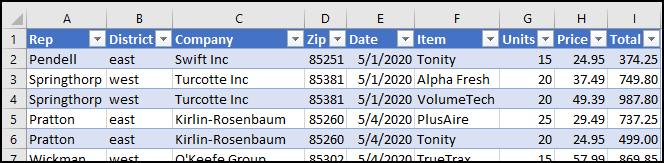
\includegraphics[width=\maxwidth{.95\linewidth}]{gfx/ch09_fig11}
	\caption{Top Of the Data Table}
	\label{09:fig11}
\end{figure}

\begin{enumerate}[resume]
	\item At \fmtRibbonButton{Table Design $ \Rightarrow $ Properties $ \Rightarrow $ Table Name} enter \fmtTyping{Sales} as the new table name. That name is entered in a text box near the left edge of the ribbon.
\end{enumerate}

In a database, columns are referred to as ``Fields'' and rows as ``Records.'' Notice that each of the fields in the data table includes a drop-down arrow. That opens a menu with filtering functions that can be applied to the database. Figure \ref{09:fig12} illustrates the filter for the \textit{Item} field.

\begin{figure}[H]
	\centering
	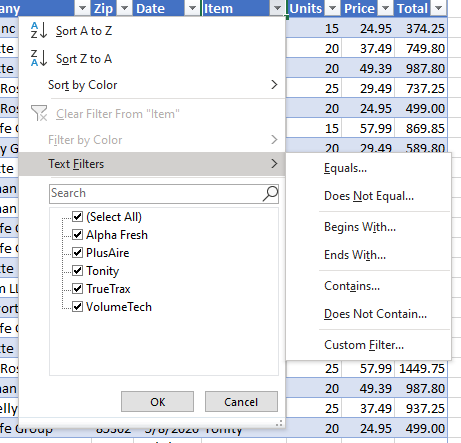
\includegraphics[width=\maxwidth{.95\linewidth}]{gfx/ch09_fig12}
	\caption{Item Filter}
	\label{09:fig12}
\end{figure}

The database can be sorted on the item field by clicking either of the top two buttons in the filter drop-down (named ``Sort A to Z'' and ``Sort Z to A''). Clicking the \fmtPopupButton{Text Filters} button opens a submenu where powerful filters can be created. Also, the checkboxes at the bottom of the popup can be used to hide or view records that match the selected item. Thus, to only see the ``Alpha Fresh'' records, uncheck all boxes except that one.

\subsection{The Database Functions}

Along with simple sorting and filtering, Excel provides the following functions that are designed to be used with a database. 

\begin{itemize}
	\item \textbf{DAVERAGE}. Calculates the average of values in a field that satisfy specified conditions.
	\item \textbf{DCOUNT}. Returns the number of cells containing numbers in a field that satisfy specified conditions.
	\item \textbf{DCOUNTA}. Returns the number of non-blank cells in a field that satisfy specified conditions.
	\item \textbf{DGET}. Returns a single value from a field that satisfy specified conditions.
	\item \textbf{DMAX}. Returns the maximum value from a field that satisfy specified conditions.
	\item \textbf{DMIN}. Returns the minimum value from a field that satisfy specified conditions.
	\item \textbf{DPRODUCT}. Calculates the product of values in a field that satisfy specified conditions.
	\item \textbf{DSTDEV}. Calculates the standard deviation (based on a sample of a population) of values in a field that satisfy specified conditions.
	\item \textbf{DSTDEVP}. Calculates the standard deviation (based on an entire population) of values in a field that satisfy specified conditions.
	\item \textbf{DSUM}. Calculates the sum of values in a field that satisfy specified conditions.
	\item \textbf{DVAR}. Calculates the variance (based on a sample of a population) of values in a field that satisfy specified conditions.
	\item \textbf{DVARP}. Calculates the variance (based on an entire population) of values in a field that satisfy specified conditions.
\end{itemize}

These functions all use similar syntax: \fmtTyping{=FuncName(Database, Field, Criteria)}. In the function, the ``FuncName'' is the name of the function, like ``DSUM.'' The database name will be ``Sales'' since that is the name of the table. The Field is one of the field names, like ``Rep'' or ``District.'' Finally, the criteria is a range that contains the factors that limit the output of the function. This is best explained with some examples.

\begin{itemize}[resume]
	\item Enter \fmtTyping{Zip} in \fmtCellLocation{K2}, \fmtTyping{85260} in \fmtCellLocation{K3}, and \fmtTyping{Sum} in \fmtCellLocation{L3}. This will set up an area where the sum of all orders sent to Zip $ 85260 $ will be calculated.
	\item Enter this formula in \fmtCellLocation{L3}: \fmtTyping{=DSUM(Sales[\#All],''Total'',K2:K3)}. Here is what the various parts of this formula mean.

	\begin{enumerate}
		\item \textbf{DSUM}. This is the ``data sum'' function that totals all of the specified data.
		\item \textbf{Sales[\#All]}. This instructs Excel to use the entire Sales data table. By using this nomenclature rather than specific cell locations (like \fmtCellLocation{A1:I69}), the formula will continue to work even if records are added to or removed from the table.
		\item \textbf{Total}. This is the field that contains the numbers to be summed. Notice that the field name is put in quote marks.
		\item \textbf{K2:K3}. This is the location of the criteria Excel will use to sum the sales amounts.
	\end{enumerate}	

	\begin{figure}[H]
		\centering
		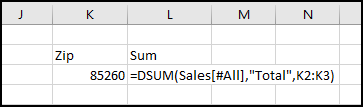
\includegraphics[width=\maxwidth{.95\linewidth}]{gfx/ch09_fig21}
		\caption{Setting Up the Data File Calculation}
		\label{09:fig21}
	\end{figure}

	\item Once the formula and criteria are entered, Excel calculates the total value of sales to that Zip and displays $ 14747.55 $.
	\item Change the Zip in \fmtCellLocation{K3} to \fmtTyping{85251}. The value in cell \fmtCellLocation{L3} will be automatically updated to $ 748.50 $, which is the total value in sales to that Zip code.
	\item Copy/paste cells \fmtCellLocation{K2:L3} to \fmtCellLocation{K5:L6}. When pasted, Excel will automatically update the criteria range in the formula to \fmtCellLocation{K5:K6}.
	\item Change the value of \fmtCellLocation{K5} to \fmtTyping{District} and \fmtCellLocation{K6} to \fmtTyping{east}. \fmtCellLocation{L6} now displays $ 22546.95 $, which is the total value of sales to the ``east'' district.
	\item Copy/paste \fmtCellLocation{K5:L6} to \fmtCellLocation{K8:L9}.
	\item Change the formula in \fmtCellLocation{L9} to calculate the average value of the total sales by changing \fmtTyping{DSUM} to \fmtTyping{DAVERAGE}. The formula in \fmtCellLocation{L9} should now be: \fmtTyping{=DAVERAGE(Sales[\#All],''Total'',K8:K9)}
	\item Change \fmtCellLocation{K8} to \fmtTyping{Rep} and \fmtCellLocation{K9} to \fmtTyping{Pratton}. \fmtCellLocation{L9} should now display $ 736.7236842 $, which is the average sale value for Pratton. The average sale for other sellers can be easily checked by entering their names in \fmtCellLocation{K9}, one at a time.
\end{itemize}

One important feature for any database lookup is the ability to specify ``Boolean'' matches; that is, a match that includes an AND term or an OR term. For example, that would answer a question like, ``What is the total value of the sales of TrueTrax made by Findlay?'' Follow these steps to create Boolean expressions.

\begin{enumerate}
	\item Copy/paste \fmtCellLocation{K8:K9} to \fmtCellLocation{K11:K12} and also paste \fmtCellLocation{K8:K9} to \fmtCellLocation{L8:L9}. Change \fmtCellLocation{K11} to \fmtTyping{Rep}, \fmtCellLocation{K12} to \fmtTyping{Findlay}, \fmtCellLocation{L11} to \fmtTyping{Item} and \fmtCellLocation{L12} to \fmtTyping{TrueTrax}.
	\item Copy/paste \fmtCellLocation{L8:L9} to \fmtCellLocation{M11:M12}. Change the formula in \fmtCellLocation{M12} to \fmtTyping{=DSUM(Sales[\#All],''Total'',K11:L12)}.
	
	\begin{figure}[H]
		\centering
		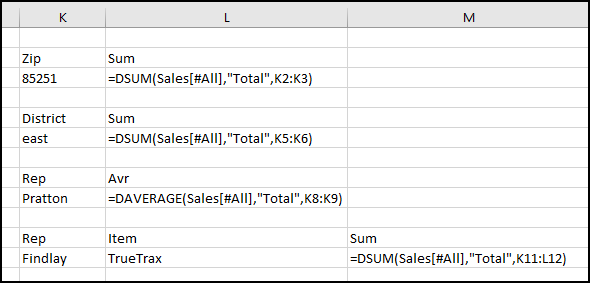
\includegraphics[width=\maxwidth{.95\linewidth}]{gfx/ch09_fig22}
		\caption{Calculating an AND Expression}
		\label{09:fig22}
	\end{figure}
	
	\item Excel displays $ 1739.7 $ in \fmtCellLocation{M12}, which is the total value of Findlay's TrueTrax sales. 
	\item Data criteria items that appear in the same row are combined with an AND, so K11:L12 would be read ``Calculate the sum of all lines that include a representative named Findlay AND an item named TrueTrax.''
	\item Note: The order of the ANDed terms is important. They must be in the same order in the criteria section as they are in the data table. Therefore, if ``Item'' were in \fmtCellLocation{K11} and ``Rep'' in \fmtCellLocation{L11} the formula would fail.
	\item Other sales representative names can be entered in cell \fmtCellLocation{K12} or other items in \fmtCellLocation{L12} to check on those sales.
	\item To combine two or more terms with an OR, place those terms on separate lines. 
	\item Copy/paste \fmtCellLocation{K11:M12} to \fmtCellLocation{K14:M15}.
	\item Rather than calculate the total value of Findlay's sales, count the number of items sold. Change \fmtCellLocation{M14} to \fmtTyping{Units Sold}.
	\item Change the formula in \fmtCellLocation{M15} to: \fmtTyping{=DSUM(Sales[\#All],''Units'',K14:L15)}. Notice that the only change to the formula is that it will sum the \textit{Units} field instead of the \textit{Total} field.
	\item To include PlusAir in this sum, enter \fmtTyping{PlusAir} in \fmtCellLocation{L16}. Then, change the formula in \fmtCellLocation{M15} to \fmtTyping{=DSUM(Sales[\#All],''Units'',K14:L16)}. Notice that the only change is to increase the criteria range to \fmtCellLocation{K14:L16}. Now, Excel will count the total number of lines that include both Findlay and TrueTrax OR Finaley and PlusAir. Excel reports that Findlay sold $ 50 $ TrueTrax OR PlusAir units.
	
	\begin{figure}[H]
		\centering
		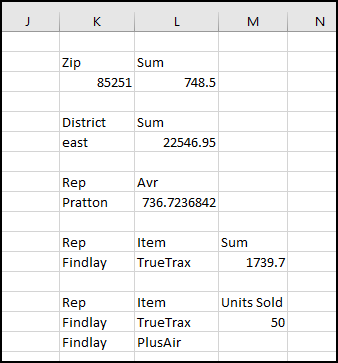
\includegraphics[width=\maxwidth{.95\linewidth}]{gfx/ch09_fig23}
		\caption{Calculating an OR Expression}
		\label{09:fig23}
	\end{figure}
\end{enumerate}

Finally, it is often desirable to set up a range for a data calculation. For example, it is possible to count the total number of Tonity sales made between May $ 5 $ and May $ 20 $.

\begin{enumerate}
	\item Enter \fmtTyping{Date} in \fmtCellLocation{K18}, \fmtTyping{Date} in \fmtCellLocation{L18} (the Date will be entered two times in the criteria), \fmtTyping{Item} in \fmtCellLocation{M18}, and \fmtTyping{Count} in \fmtCellLocation{N18}.
	\item Enter \fmtTyping{>=5/10/2020} in \fmtCellLocation{K19}, \fmtTyping{<=5/20/2020} in \fmtCellLocation{L19}, and \fmtTyping{Tonity} in \fmtCellLocation{M19}.
	\item Enter this formula in \fmtCellLocation{N19}: \fmtTyping{=DCOUNT(Sales[\#All],''Total'',K18:M19)}. Notice that this is a DCOUNT formula, so the number of lines that contain a Tonity item sold between $ 5/10/2020 $ and $ 5/20/2020 $ (inclusive) will be counted.
	
	\begin{figure}[H]
		\centering
		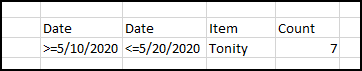
\includegraphics[width=\maxwidth{.95\linewidth}]{gfx/ch09_fig24}
		\caption{Specifying a Date Range}
		\label{09:fig24}
	\end{figure}

	\item Excel reports seven Tonity sales were made between the two specified dates.

\end{enumerate}

Creating a data table is easy in Excel, then the data formulas make it easy to create complex calculations by simply specifying the criteria.
	
\begin{center}
	\begin{tkwbox}{Key Take-Aways}
		\textbf{Database Functions}
		\\
		\begin{itemize}
			\setlength{\itemsep}{0pt}
			\setlength{\parskip}{0pt}
			\setlength{\parsep}{0pt}
			
			\item Set up the database functions by creating a data table.
			\item Use any of the ``D...'' functions to easily count, sum, or statistically analyze a data table using complex Boolean operations. 
			
		\end{itemize}
	\end{tkwbox}
\end{center}

\section{More Functions}

\begin{center}
	\begin{objbox}{Learning Objectives}
		\begin{itemize}
			\setlength{\itemsep}{0pt}
			\setlength{\parskip}{0pt}
			\setlength{\parsep}{0pt}
			
			\item one
			
		\end{itemize}
	\end{objbox}
\end{center}

\subsection{Functions for Beginners}

\begin{enumerate}
	\item Sum
	\item Average
	\item If
	\item Sumif
	\item Countif
	\item Concatenate
	\item Right/Left
	\item Search
	\item Min/Max
	\item Trim
\end{enumerate}

\subsection{Functions for Advanced Users}

\begin{enumerate}
	\item Today/Now/Date
	\item Rand
	\item VLookup
	\item Index Match
	\item Upper/Lower/Proper
	\item AND/OR
	\item NOT
	\item Text To Columns
	\item Round
	\item Time (Hour, Minute, Second)
\end{enumerate}

\begin{center}
	\begin{tkwbox}{Key Take-Aways}
		\textbf{x}
		\\
		\begin{itemize}
			\setlength{\itemsep}{0pt}
			\setlength{\parskip}{0pt}
			\setlength{\parsep}{0pt}
			
			\item one
			
		\end{itemize}
	\end{tkwbox}
\end{center}

\section{Get \& Transform}

\begin{center}
	\begin{objbox}{Learning Objectives}
		\begin{itemize}
			\setlength{\itemsep}{0pt}
			\setlength{\parskip}{0pt}
			\setlength{\parsep}{0pt}
			
			\item one
			
		\end{itemize}
	\end{objbox}
\end{center}

(\fmtExcelNew{365} Note: this is called Power Query in Excel 365.)

To use Get \& Transform in Excel, you create a query in your workbook. A query enables you to connect to, preview, and transform data from a wide variety of available data sources. You can then load that transformed data into a table, or into the built-in Data Model in Excel, and even refresh that data later on. You can also edit the query and share it with other people who are working on the same project.

To create a query in Excel, use the Data tab in the ribbon, then select the Get Data button from the Get \& Transform Data ribbon group. From there, choose your data source. 

Click \fmtRibbonButton{Data $ \Rightarrow $ Get \& Transform Data $ \Rightarrow $ Get Data}.

If you select Load, the data source is brought directly into Excel as is. If you select the Transform Data option, that will launch Query Editor.

\begin{center}
	\begin{tkwbox}{Key Take-Aways}
		\textbf{x}
		\\
		\begin{itemize}
			\setlength{\itemsep}{0pt}
			\setlength{\parskip}{0pt}
			\setlength{\parsep}{0pt}
			
			\item one
			
		\end{itemize}
	\end{tkwbox}
\end{center}

\section{Statistics}

\begin{center}
	\begin{objbox}{Learning Objectives}
		\begin{itemize}
			\setlength{\itemsep}{0pt}
			\setlength{\parskip}{0pt}
			\setlength{\parsep}{0pt}
			
			\item one
			
		\end{itemize}
	\end{objbox}
\end{center}







Excel includes an \textit{Analysis Toolpak} that contains $ 19 $ advanced statistics and engineering functions, but it is considered an Add-in and must be activated before it can be used.

\begin{enumerate}
	\item Click \fmtRibbonTab{File} to open the backstage view.
	\item In the backstage view, click \fmtRibbonButton{Options} at the bottom of the left-hand menu.
	
\end{enumerate}

\begin{figure}[H]
	\centering
	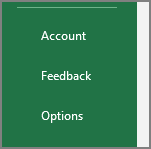
\includegraphics[width=\maxwidth{.95\linewidth}]{gfx/ch09_fig35}
	\caption{The Options Button in the Backstage View}
	\label{09:fig35}
\end{figure}

\begin{enumerate}[resume]	
	
	\item Click \fmtPopupButton{Add-ins} in the left-hand menu of the \fmtPopupBox{Excel Options} pop-up box.
	\item Select \fmtPopupBox{Excel Add-ins} in the drop-down menu at the bottom of the \fmtPopupBox{Add-ins} tab.
	\item Click \fmtPopupButton{Go}.
	
\end{enumerate}

\begin{figure}[H]
	\centering
	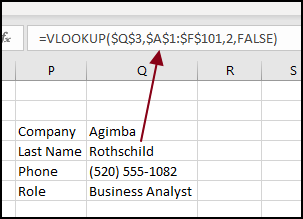
\includegraphics[width=\maxwidth{.95\linewidth}]{gfx/ch09_fig36}
	\caption{The Add-ins Manager}
	\label{09:fig36}
\end{figure}

\begin{enumerate}[resume]	
	
	\item Click the checkbox beside \fmtPopupBox{Analysis Toolpak Add-in} in the \fmtPopupBox{Add-ins} pop-up box.
	
\end{enumerate}

\begin{figure}[H]
	\centering
	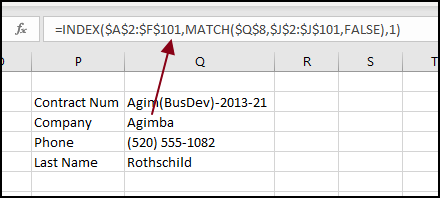
\includegraphics[width=\maxwidth{.95\linewidth}]{gfx/ch09_fig37}
	\caption{Activating The Analysis Toolpak Add-In}
	\label{09:fig37}
\end{figure}

\begin{enumerate}[resume]	
	\item Click \fmtPopupButton{OK}.
\end{enumerate}

Notice that there is a new \fmtRibbonButton{Data Analysis} button at \fmtRibbonButton{Data $ \Rightarrow $ Analyze}.

\begin{figure}[H]
	\centering
	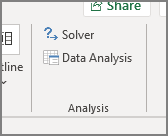
\includegraphics[width=\maxwidth{.95\linewidth}]{gfx/ch09_fig38}
	\caption{The Data Analysis Button}
	\label{09:fig38}
\end{figure}







\begin{center}
	\begin{tkwbox}{Key Take-Aways}
		\textbf{x}
		\\
		\begin{itemize}
			\setlength{\itemsep}{0pt}
			\setlength{\parskip}{0pt}
			\setlength{\parsep}{0pt}
			
			\item one
			
		\end{itemize}
	\end{tkwbox}
\end{center}

\section{Macros}

\begin{center}
	\begin{objbox}{Learning Objectives}
		\begin{itemize}
			\setlength{\itemsep}{0pt}
			\setlength{\parskip}{0pt}
			\setlength{\parsep}{0pt}
			
			\item Automate simple tasks with a macro.
			
		\end{itemize}
	\end{objbox}
\end{center}

\fmtRibbonButton{View $ \Rightarrow $ Macros $ \Rightarrow $ Macros} allows users to automate repetitive tasks. The top part of the button will open the \fmtPopupBox{View Macros} dialog box and the bottom half reveals options for macros. 

\begin{enumerate}
	\item Open a new blank workbook. (\textit{Note}: the macro is placed in a new workbook so it does not accidentally interfere with the exercises in any other workbook.)
	\item Click \fmtCellLocation{A1} to select that cell.
	\item Click \fmtRibbonButton{View $ \Rightarrow $ Macros $ \Rightarrow $ Macros} (be sure to click the small arrow at the bottom of the \fmtRibbonButton{Macros} button).
	\item Select \fmtPopupButton{Use Relative References}.
	\item Select \fmtPopupButton{Record Macro}.
	\item Name the macro \fmtTyping{MyName}.
	\item Click in the \fmtPopupBox{Shortcut Key} box and type \fmtKeystroke{Shift} $ + $ \fmtKeystroke{Q}.
	\item Store the macro in this workbook.
	\item Enter this description: \fmtTyping{Inserts my name}.
\end{enumerate}

\begin{figure}[H]
	\centering
	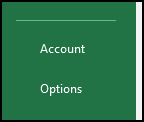
\includegraphics[width=\maxwidth{.95\linewidth}]{gfx/ch09_fig50}
	\caption{The Record Macro Settings Box}
	\label{09:fig50}
\end{figure}

\begin{enumerate}[resume]	
	\item Click \fmtPopupButton{OK}.
	\item Type your first and last name and press \fmtKeystroke{Enter}.
	\item Click \fmtRibbonButton{View $ \Rightarrow $ Macros $ \Rightarrow $ Macros} (be sure to click the small arrow at the bottom of the \fmtRibbonButton{Macros} button).
	\item Select \fmtPopupButton{Stop Recording}.
\end{enumerate}

Select another cell on the worksheet and press \fmtKeystroke{Ctrl} $ + $ \fmtKeystroke{Shift} $ + $ \fmtKeystroke{Q}. Remember that relative references were activated for the macro, otherwise the name would have always been created in cell \fmtCellLocation{A1} (the original cell) instead of the current cell.

\begin{enumerate}
	\item Click \fmtRibbonButton{View $ \Rightarrow $ Macros $ \Rightarrow $ Macros} (be sure to click the top of the \fmtRibbonButton{Macros} button).
	\item This opens the Macro manager dialog where macros can be edited, deleted, or have various options set.
\end{enumerate}

\begin{figure}[H]
	\centering
	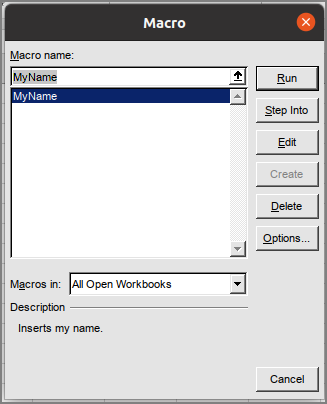
\includegraphics[width=\maxwidth{.95\linewidth}]{gfx/ch09_fig51}
	\caption{The Macro Manager Box}
	\label{09:fig51}
\end{figure}

\begin{enumerate}[resume]	
	\item Click \fmtPopupButton{Cancel} to close the Macro manager.
\end{enumerate}

Remember that all workbooks containing macros must be saved using the ``macro-enabled'' option (that creates a file extension of \textit{.xlsm}). Figure \ref{09:fig52} shows a drop-down menu at the bottom right corner of the \fmtPopupBox{Save-As} screen where \fmtPopupButton{Excel Macro-Enabled Workbook} must be selected. 

\begin{figure}[H]
	\centering
	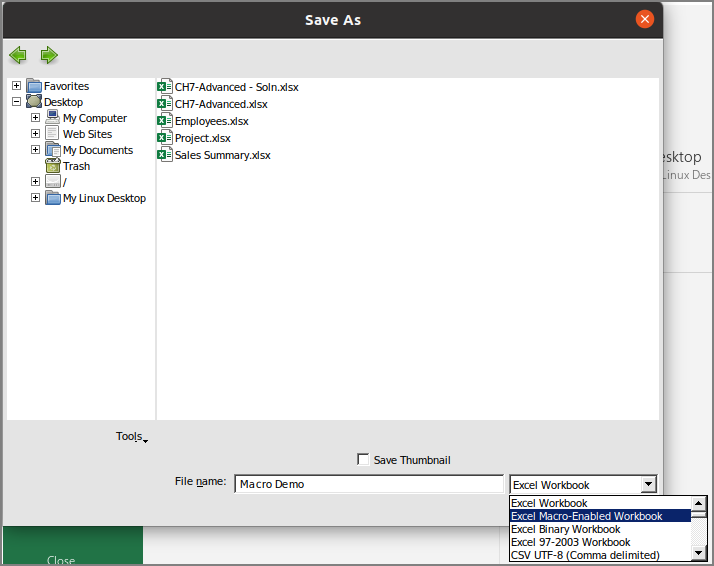
\includegraphics[width=\maxwidth{.95\linewidth}]{gfx/ch09_fig52}
	\caption{Saving a Workbook With a Macro}
	\label{09:fig52}
\end{figure}

Since this macro will not be reused in the future, close the workbook without saving.

\begin{center}
	\begin{tkwbox}{Key Take-Aways}
		\textbf{Using Excel Macros}
		\\
		\begin{itemize}
			\setlength{\itemsep}{0pt}
			\setlength{\parskip}{0pt}
			\setlength{\parsep}{0pt}
			
			\item Macros automate simple tasks to save time in data entry.
			\item Workbooks containing macros must be saved with the ``Macro-Enabled'' setting.
			
		\end{itemize}
	\end{tkwbox}
\end{center}

\section{Excel Preferences}

\begin{center}
	\begin{objbox}{Learning Objectives}
		\begin{itemize}
			\setlength{\itemsep}{0pt}
			\setlength{\parskip}{0pt}
			\setlength{\parsep}{0pt}
			
			\item one
			
		\end{itemize}
	\end{objbox}
\end{center}

Lorem

\begin{center}
	\begin{tkwbox}{Key Take-Aways}
		\textbf{x}
		\\
		\begin{itemize}
			\setlength{\itemsep}{0pt}
			\setlength{\parskip}{0pt}
			\setlength{\parsep}{0pt}
			
			\item one
			
		\end{itemize}
	\end{tkwbox}
\end{center}



\section{Chapter Practice}

\subsection{Project Team Analysis}

\textit{Data file: PR7-Data.csv}


\section{Scored Assessment}

\subsection{Employee Analysis}

\textit{Data file: SC7-Data.csv}

